\documentclass{beamer}
%
% Choose how your presentation looks.
%
% For more themes, color themes and font themes, see:
% http://deic.uab.es/~iblanes/beamer_gallery/index_by_theme.html
%
\mode<presentation>
{
  \usetheme{Warsaw}      % or try Darmstadt, Madrid, Warsaw, ... (default)
  \usecolortheme{crane} % or try albatross, beaver, crane, ... (deafult)
  \usefonttheme{serif}  % or try serif, structurebold, ... (deafult)
  \setbeamertemplate{navigation symbols}{}
  \setbeamertemplate{caption}[numbered]
  \setbeameroption{show notes} %un-comment to see the notes
} 

\usepackage[english]{babel}
\usepackage[utf8x]{inputenc}
\usepackage{wrapfig}
\usepackage{multimedia}

\title[Simple Flocking]{Simulation of a Flocking Model}
\author{Lorenzo Sani}
\institute{Università degli Studi di Bologna}
\date{\today}

\begin{document}

\begin{frame}
  \titlepage
\end{frame}

% Uncomment these lines for an automatically generated outline.
%\begin{frame}{Outline}
%  \tableofcontents
%\end{frame}

\section{Introduction}

\begin{frame}{Introduction}
\begin{minipage}[0.95\textheight]{\textwidth}
\begin{columns}[T]
\begin{column}{0.30\textwidth}
\begin{itemize}
  \item Emergence
  \vspace{0.2cm}
  \item Internal interactions \\and scale  laws
  \vspace{0.2cm}
  \item Dynamical phase transitions
  \vspace{0.2cm}
  \item Limiting process
\end{itemize}
\end{column}
\begin{column}{0.65\textwidth}
	\vspace*{0.6cm}
	\centering
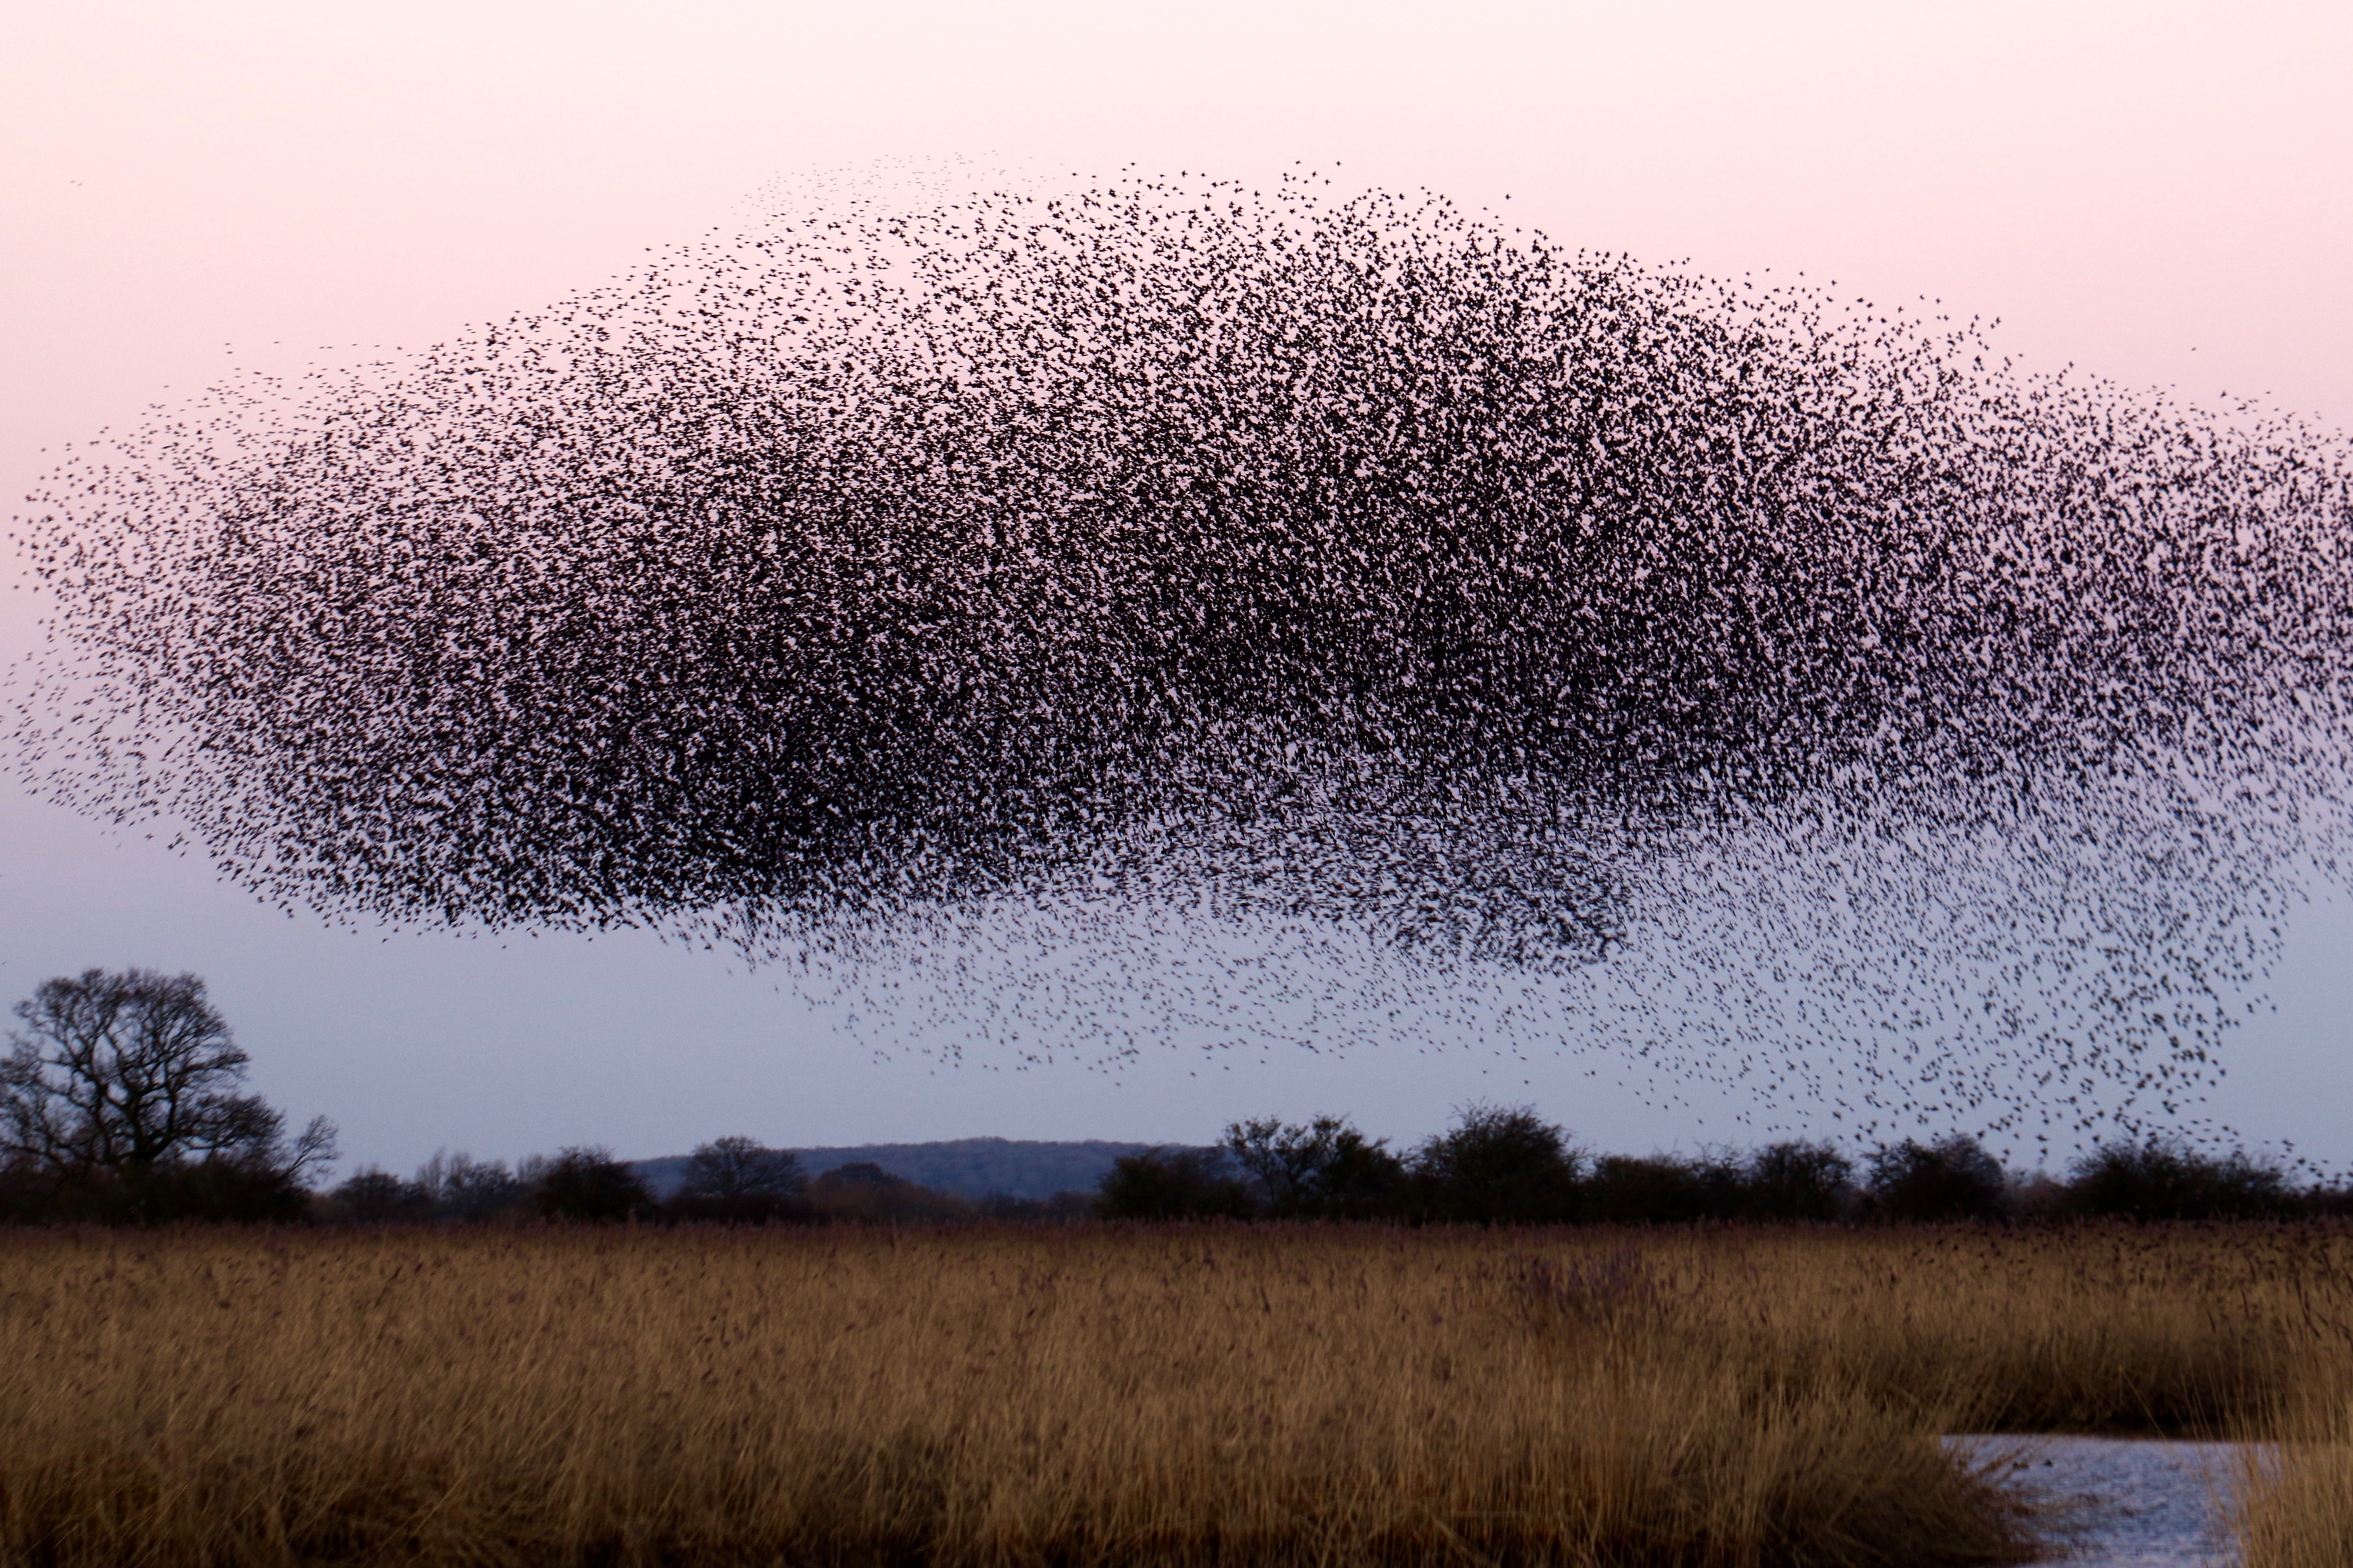
\includegraphics[width=\textwidth, keepaspectratio]{../images/flock_image.jpeg}
\end{column}
\end{columns}
\end{minipage}
\end{frame}

\section{The Model}
\begin{frame}{Assumptions}
	\begin{minipage}[0.95\textheight]{\textwidth}
	\begin{columns}[T]
	\begin{column}{0.40\textwidth}
		\begin{itemize}
		\item Convergence to a global critical state
		\vspace{0.5cm}
		\item Global interaction between birds
		\vspace{0.5cm}
		\item Interaction depending on visual perception
		\end{itemize}
	\end{column}
	\begin{column}{0.50\textwidth}
		\begin{center}
		\movie[loop]{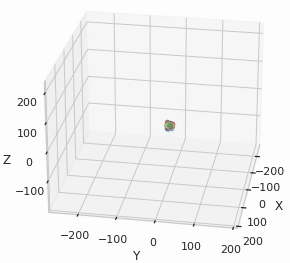
\includegraphics[width=\textwidth, keepaspectratio]{../images/screen_for_ani_N50.mp4.png}}{../images/animation_N50_crop.mp4}
		\end{center}
	\end{column}
	\end{columns}
	\end{minipage}
\end{frame}
\begin{frame}{Weighting Function}
	\begin{equation}
		v_i(t+h)-v_i(t)=h\sum_{j=1}^k a_{ij}(v_j(t)-v_i(t))\nonumber
	\end{equation}
  \vspace{1cm}
	\begin{equation}
		a_{ij}=\eta(x_i,x_j)=\frac{H}{\big(\sigma^2+\left\Vert x_i - x_j \right\Vert^2\big)^{\beta}}\nonumber
	\end{equation}
\end{frame}
\begin{frame}{Complex Network Theory}
	\begin{itemize}
		\item Adjacency matrix $A_x = \lbrace a_{ij}\rbrace=\bigg\lbrace\frac{H}{(\sigma^2+\left\Vert x_i - x_j \right\Vert^2)^{\beta}}\bigg\rbrace\nonumber$
		\vspace{0.5cm}
		\item Degree matrix $D_x = diag(d_1,...d_k) \text{, where } d_i=\bigg(\sum_{j\leq k}a_{ij}\bigg)$
		\vspace{0.5cm}
		\item Laplacian matrix $L_x = D_x - A_x$
	\end{itemize}
\end{frame}
\begin{frame}{Discrete and Continuous Case}
	\begin{minipage}[0.95\textheight]{\textwidth}
	\begin{columns}[T]
	\begin{column}{0.5\textwidth}
		\begin{itemize}
		  \item Discrete
		  \vspace{0.5cm}
		\end{itemize}
		\begin{align}
			&x(t+h) = x(t) + hv(t)\nonumber\\
			&v(t+h) = (Id -hL_x)v(t)\nonumber
		\end{align}
	\end{column}
	\begin{column}{0.5\textwidth}
		\begin{itemize}
		  \item Continuous
		  \vspace{0.5cm}
		\end{itemize}
		\begin{align}
			&\dot{x} = v\nonumber\\
			&\dot{v} = -L_xv\nonumber
		\end{align}
	\end{column}
	\end{columns}
	\end{minipage}
\end{frame}
\begin{frame}{Theorem}
	\begin{itemize}
		\item for $\beta \le 1/2$ when $t\rightarrow\infty$
		\begin{itemize}
			\item velocities $v_i(t)\rightarrow\widehat{v}\in\mathbf{E}$ common
			\item distances $x_i-x_j\rightarrow\widehat{x_{ij}}$ for $\forall i,j\leq k$
		\end{itemize}
		\vspace{0.5cm}
		\item for $\beta > 1/2$ when $t\rightarrow\infty$
		\begin{itemize}
			\item convergence is reached under special initial conditions
		\end{itemize}
	\end{itemize}
\end{frame}

\section{Results}
\begin{frame}{Representative convergence}
	\begin{minipage}[0.95\textheight]{\textwidth}
	\begin{columns}[T]
	\begin{column}{0.50\textwidth}
	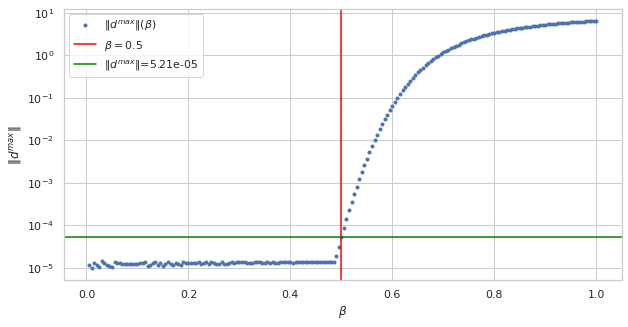
\includegraphics[width=\textwidth, keepaspectratio]{../images/d_conv.png}
	\end{column}
	\begin{column}{0.50\textwidth}
	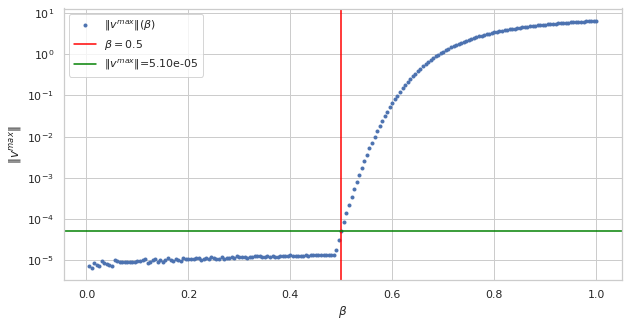
\includegraphics[width=\textwidth, keepaspectratio]{../images/v_conv.png}
	\end{column}
	\end{columns}
	\end{minipage}
	\begin{center}
		Parameters: $k=100$, $\sigma=1$, $\beta$ varying\\
		max \# iterations = 5000, accepted convergence at $10^{-5}$
	\end{center}
\end{frame}
\begin{frame}{Trend of Convergence increasing $k$}
	\begin{minipage}[0.95\textheight]{\textwidth}
	\begin{columns}[T]
	\begin{column}{0.50\textwidth}
	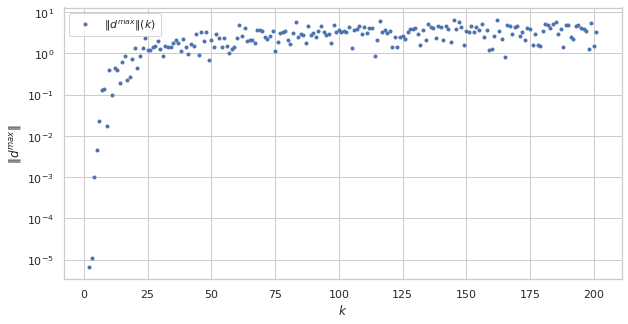
\includegraphics[width=\textwidth, keepaspectratio]{../images/d_conv_N.png}
	\end{column}
	\begin{column}{0.50\textwidth}
	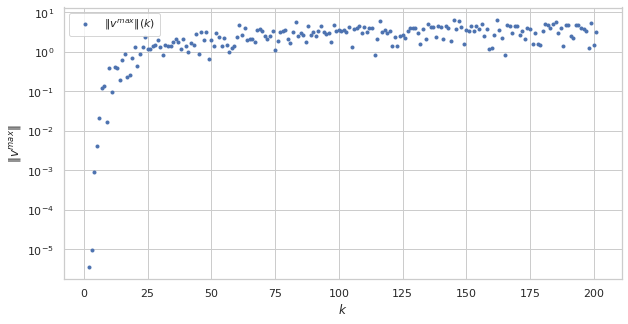
\includegraphics[width=\textwidth, keepaspectratio]{../images/v_conv_N.png}
	\end{column}
	\end{columns}
	\end{minipage}
	\begin{center}
		Parameters: $k$ varying, $\sigma=1$, $\beta=1/2$\\
		max \# iterations = 100
	\end{center}
\end{frame}
\begin{frame}{Influence of $k$}
	\begin{minipage}[0.95\textheight]{\textwidth}
	\begin{columns}[T]
	\begin{column}{0.50\textwidth}
	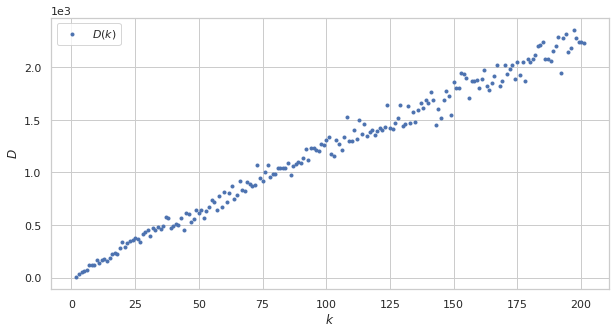
\includegraphics[width=\textwidth, keepaspectratio]{../images/D_N.png}
	\end{column}
	\begin{column}{0.50\textwidth}
	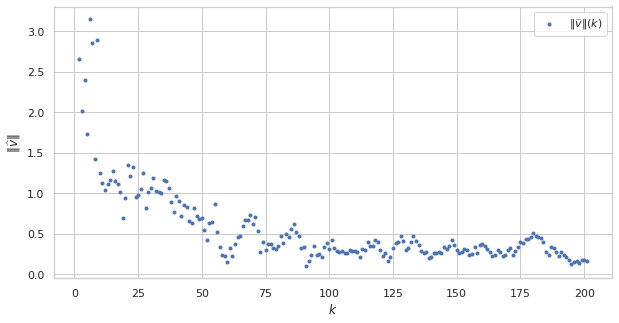
\includegraphics[width=\textwidth, keepaspectratio]{../images/v_N.png}
	\end{column}
	\end{columns}
	\end{minipage}
	\begin{center}
		Parameters: $k$ varying, $\sigma=1$ fixed, $\beta=0.4$\\
		max \# iterations $\propto$ $k$ to let the system reach convergence
	\end{center}
\end{frame}
\begin{frame}{Influence of $\sigma$}
	\begin{minipage}[0.95\textheight]{\textwidth}
	\begin{columns}[T]
	\begin{column}{0.50\textwidth}
	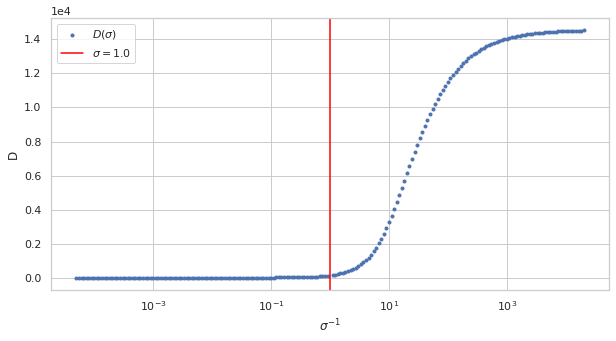
\includegraphics[width=\textwidth, keepaspectratio]{../images/D_sigma.png}
	\end{column}
	\begin{column}{0.50\textwidth}
	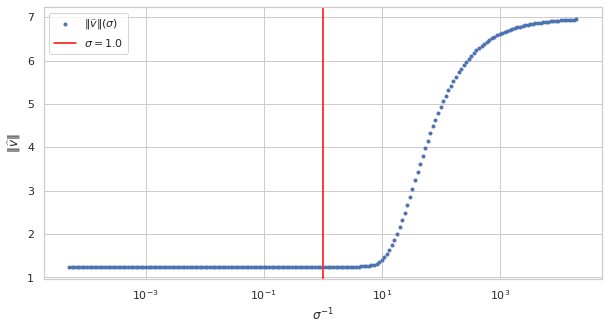
\includegraphics[width=\textwidth, keepaspectratio]{../images/v_sigma.png}
	\end{column}
	\end{columns}
	\end{minipage}
	\begin{center}
		Parameters: $k=100$, $\sigma$ varying, $\beta=0.4$\\
		max \# iterations = 1000
	\end{center}
\end{frame}

\section{Conclusions}
\begin{frame}{Conclusions}
	\begin{itemize}
		\item Convergence not so sharp
		\vspace{0.5cm}
		\item Does not converge at very large $k$, unless the convergence criteria are tuned accordingly
		\vspace{0.5cm}
		\item Critical state fulfills the expectations
		\vspace{0.5cm}
		\item Good behavior of the characteristics of the flocking state
	\end{itemize}
\end{frame}

\begin{frame}{}
	The end,\\
	Thanks for the attention
\end{frame}

\end{document}